\documentclass[12pt]{article}
\usepackage{tikz}
\usepackage{amsmath}
\usepackage{amsthm}
\usepackage{amssymb}
\usepackage{enumitem}
\begin{document}
\title{COSC221 Assignment 3}
\author{Rin Meng \\ Student ID: 51940633}
\maketitle


\begin{enumerate}[label=Part \Alph*)]
    \item
    \begin{proof}[Proof]
        By induction on $n \in \mathbb{Z}^{+}$. Here, we choose $\mathbb{Z}^{+}$ because it is intuitive to have a positive integer of $n \times n$ chessboard. 
        
        \textbf{Remark:} $\mathbb{Z}^{+}$ is the set of all positive integers; $\mathbb{Z}^{+} = \{1, 2, 3, \ldots, n\}_{n \rightarrow \infty}$.
        
        \textbf{Base Case:} $n = 1$
        
        $S(1) = 1 \times 1$ chessboard, so there exists one cell only on that chessboard, which makes it the top-left and the bottom-left cell, where the rook starts and ends at the same cell. Hence, there exists the rook's tour, even if $n = 1$ is a little bit trivial.
        
        \textbf{Inductive Hypothesis:} If our constructed $S(n)$ holds, then there exists some $n \in \mathbb{Z}^{+}$ such that it satisfies $S(n + 1)$ as well.
        
        \textbf{Inductive Step:} $n \rightarrow n + 1$
        
        $S(n+1) = (n + 1) \times (n + 1)$ chessboard. By the given information on page 234 for rook's tour and rook's move, we let $(r, c, x) \in \mathbb{Z}^{+}$, then it is true that rook can start at $\langle r, c \rangle$. Then for $n \times n$ chessboard to $(n + 1) \times (n + 1)$ chessboard, there are two possible movement,
        
        Vertical movement $\Rightarrow \langle r, c \pm x \rangle \rightarrow \langle r, n+1 \rangle$, so this means that $c \pm x = n + 1 \Leftrightarrow c = n + 1 \pm x$
        
        Horizontal movement $\Rightarrow \langle r \pm x, c \rangle \rightarrow \langle n+1, c \rangle$, so this also means that $r \pm x = n + 1 \Leftrightarrow r = n + 1 \pm x$
        
        Now, we know that, if we let
        $$x = min(\mathbb{Z}^{+}) = 1$$
        and, 
        $$min(r) = min(c) = n + 1 - x$$
        therefore,
		$$min(r) = min(c) = n + 1 - 1 = n$$
        Then, our movement for both vertical and horizontal are both within the bounds of $\mathbb{Z}^{+}$, as we said above, $n \in \mathbb{Z}^{+}$. Now, let these coordinates be true that $\langle 1, 1 \rangle \Rightarrow $ top-left, $\langle n + 1, 1 \rangle \Rightarrow $ top-right, $\langle 1, n + 1 \rangle \Rightarrow $ bottom-left and, $\langle n + 1, n + 1 \rangle \Rightarrow $ bottom-right. 
        
         Now to traverse through the board, there are two possible cases:
        
        \textbf{Case $\boldsymbol{\alpha}$:} $(n + 1) \times (n + 1)$ chessboard where $(n + 1) \in \mathbb{Z}_{\text{even}}$
        
        Then if we let rook start at $\langle 1, 1 \rangle $, then we follow a horizontal ``zig-zag" pattern below:
        
        $(1, 1) \rightarrow (2, 1) \rightarrow \ldots \rightarrow (n, 1) \rightarrow \underbrace{(n + 1, 1)}_{\downarrow}$
        
		$\underbrace{(1, 2)}_{\downarrow} \leftarrow (2, 2) \leftarrow \ldots \leftarrow  (n, 2) \leftarrow (n + 1, 2)$
		
		$(1, 3) \rightarrow (2, 3) \rightarrow \ldots \rightarrow  (n, 3) \rightarrow \underbrace{(n + 1, 3)}_{\downarrow}$
		
		$\hspace{190pt}\vdots\hspace{11pt}$
		
		$(1, n + 1) \leftarrow (2, n + 1) \leftarrow \ldots \leftarrow (n + 1, n + 1)$
		
		By this visual, we can clearly see that the rook arrives at the left side every time $c \in \mathbb{Z}_{\text{even}}$, so it is entirely possible that the rook can end up on the bottom-left side, because $c = (n + 1) \in \mathbb{Z}_{\text{even}}^{+}$.
 
        \textbf{Case $\boldsymbol{\beta}$:} $(n + 1) \times (n + 1)$ chessboard where $(n + 1) \in \mathbb{Z}_{\text{odd}}^{+}$
        
        Then if we let rook start at $\langle 1, 1 \rangle $, then we follow a vertical ``zig-zag" pattern below:
        
        $\underbrace{(1, 1)}_{\downarrow} \quad\;\; (2, 1) \rightarrow \underbrace{(\ldots)}_{\downarrow} \quad\;\; (n, 1) \rightarrow \underbrace{(n + 1, 1)}_{\downarrow}$
        
		$\underbrace{\vdots}_{\downarrow} \quad\quad \overbrace{\vdots}^{\uparrow} \quad\;\; \underbrace{\vdots}_{\downarrow} \quad\;\;  \overbrace{(n, \vdots )}^{\uparrow} \quad\;\; \underbrace{(n + 1, 2)}_{\downarrow}$
		
		$(1, n) \rightarrow \overbrace{(2, n)}^{\uparrow} \quad\; (\ldots) \rightarrow \overbrace{(n, n)}^{\uparrow} \quad\;\; \underbrace{(n + 1, n)}_{\downarrow}$
		
		$\hspace{200pt}\vdots\hspace{11pt}$
		
		$(1, n + 1) \leftarrow (2, n + 1) \leftarrow \ldots \leftarrow (n + 1, n + 1)$
		
		
		By this visual, we can clearly see that whenever $r \in \mathbb{Z}_{\text{odd}}$, it will be making a downwards movement, so since $(n + 1) \in \mathbb{Z}_{\text{odd}}^{+}$, we know that $n \in \mathbb{Z}_{\text{even}}^{+}$, that means that it will be making an upwards movement so that it can turn right towards $(n + 1, 1)$ where it can start moving down again. Note that we have never really visited $c = n + 1$ for these traversal, so let it be known that, after reaching $(n + 1, n + 1)$, it can go directly to $(1, n+1)$, where the rook will be at the bottom-left of the chessboard.
        
        $\therefore$ By mathematical induction, and by \textbf{Case} $\boldsymbol{\alpha}$ and $\boldsymbol{\beta}$, it is true that the rook's tour exists for the $n \times n$ chessboard, for some $n \in \mathbb{Z}^{+}$.
        
    \end{proof}
    
    \item \textbf{11.36} We know that in a simple graph,
	$$directed \Rightarrow density = \frac{|E|}{\frac{n(n-1)}{2}} = \frac{2|E|}{n(n-1)}$$
	$$undirected \Rightarrow density =  \frac{|E|}{n(n-1)}$$
	Where $n$ is the vertex or node, and $|E|$ is the edges.
	
	As a function of n the density of an n-node path means, $|E| \Rightarrow (n - 1)$, where $n$ is vertices, so we have,
	$$f(n) = \frac{2(n-1)}{n(n-1)} = \frac{2}{n}$$
	\textbf{11.37} As a function of n the density of an n-node cycle means, $|E| \Rightarrow n$, where $n$ is vertices, so we have,
	
	$$f(n) = \frac{2n}{n(n-1)} = \frac{2}{n - 1}$$
	
	\textbf{11.38} As a function of n the density of a graph that consists of $\frac{n}{3}$ disconnected triangles, $|E| \Rightarrow n$, where $n$ is vertices, so we have,
	
	$$f(n) = \frac{2n}{n(n-1)} = \frac{2}{n - 1}$$
	
	which is essentially the same as a cycle.
		
	\item \textbf{Remark:} Let it be known that clique 1, clique 2 and clique 3 represents the ``clusters" of nodes from left to right respectively in \textbf{Figure 11.33d}
	
	\textbf{11.54} We can see that each ``clusters" or cliques represents its own movie, then there must be at least, 3 movies, but it is also shown that there is two curves on the top of the graph, where the actor from the clique 3, knows actor from clique 1 and clique 2. which means that there must exists at least another 2 movies. Therefore, there must exists, at the minimum, five movies that could be generated by this collaboration network.
	
	
	
	\textbf{11.55} No, it is uncertain. It is entirely possible that there are more than 5 movies generated in this graph because each cliques can have its own subset, where the actors are in another movie different than the minimum 5 movies.
    
    \item 
    \textbf{11.95}
    \begin{proof}
    By counterexample, assume $G$ is a bipartite graph where,
    $$G = \langle L \cup R, E \rangle$$
    and where, $|L| = |R|$, so we can take, $L = \{1, 2\}$ and $R = \{3, 4\}$ and since all nodes from $L$ and $R$ has at least one neighbours, we can construct $G$ such that $E = \{\{1,3\}, \{2,4\}\}$, visually:
    
    
	\begin{center}
	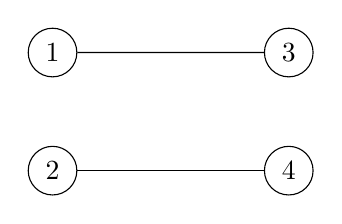
\begin{tikzpicture}[scale=1.5]
    \tikzset{vertex/.style = {shape=circle,draw,minimum size=1.5em}}
    
    % Vertices in the left set L
    \foreach \pos/\name in {{(0,1)/1}, {(0,0)/2}}
        \node[vertex] (L\name) at \pos {$\name$};
    
    % Vertices in the right set R
    \foreach \pos/\name in {{(2,1)/3}, {(2,0)/4}}
        \node[vertex] (R\name) at \pos {$\name$};
    
    % Edges between vertices
    \foreach \source/\target in {L1/R3, L2/R4}
        \draw (\source) -- (\target);
	\end{tikzpicture}
	\end{center}
	
	and we can see that the graph we made, $G$, consists of two disjoint sets which is absurd, because the original statement say that it is connected.
	
	$\therefore$ It is disproved that if $G = \langle L \cup R, E \rangle$ where $G$ is a bipartite graph with $|L| = |R|$, then it is impossible for $G$ to be a connected graph, if there is at minimum, one neighbour for every node in $L$ and $R$.x`
    \end{proof}
\end{enumerate}


End of Assignment 3.

\end{document}
